\documentclass[journal,12pt,twocolumn]{IEEEtran}

\usepackage{setspace}
\usepackage{gensymb}

\singlespacing


\usepackage[cmex10]{amsmath}

\usepackage{amsthm}

\usepackage{mathrsfs}
\usepackage{txfonts}
\usepackage{stfloats}
\usepackage{bm}
\usepackage{cite}
\usepackage{cases}
\usepackage{subfig}

\usepackage{longtable}
\usepackage{multirow}

\usepackage{enumitem}
\usepackage{mathtools}
\usepackage{steinmetz}
\usepackage{tikz}
\usepackage{circuitikz}
\usepackage{verbatim}
\usepackage{tfrupee}
\usepackage[breaklinks=true]{hyperref}
\usepackage{graphicx}
\usepackage{tkz-euclide}
\usepackage{float}

\usetikzlibrary{calc,math}
\usepackage{listings}
    \usepackage{color}                                            %%
    \usepackage{array}                                            %%
    \usepackage{longtable}                                        %%
    \usepackage{calc}                                             %%
    \usepackage{multirow}                                         %%
    \usepackage{hhline}                                           %%
    \usepackage{ifthen}                                           %%
    \usepackage{lscape}     
\usepackage{multicol}
\usepackage{chngcntr}

\DeclareMathOperator*{\Res}{Res}

\renewcommand\thesection{\arabic{section}}
\renewcommand\thesubsection{\thesection.\arabic{subsection}}
\renewcommand\thesubsubsection{\thesubsection.\arabic{subsubsection}}

\renewcommand\thesectiondis{\arabic{section}}
\renewcommand\thesubsectiondis{\thesectiondis.\arabic{subsection}}
\renewcommand\thesubsubsectiondis{\thesubsectiondis.\arabic{subsubsection}}


\hyphenation{op-tical net-works semi-conduc-tor}
\def\inputGnumericTable{}                                 %%

\lstset{
%language=C,
frame=single, 
breaklines=true,
columns=fullflexible
}
\begin{document}
\newtheorem{theorem}{Theorem}[section]
\newtheorem{problem}{Problem}
\newtheorem{proposition}{Proposition}[section]
\newtheorem{lemma}{Lemma}[section]
\newtheorem{corollary}[theorem]{Corollary}
\newtheorem{example}{Example}[section]
\newtheorem{definition}[problem]{Definition}

\newcommand{\BEQA}{\begin{eqnarray}}
\newcommand{\EEQA}{\end{eqnarray}}
\newcommand{\define}{\stackrel{\triangle}{=}}
\bibliographystyle{IEEEtran}
\providecommand{\mbf}{\mathbf}
\providecommand{\pr}[1]{\ensuremath{\Pr\left(#1\right)}}
\providecommand{\qfunc}[1]{\ensuremath{Q\left(#1\right)}}
\providecommand{\sbrak}[1]{\ensuremath{{}\left[#1\right]}}
\providecommand{\lsbrak}[1]{\ensuremath{{}\left[#1\right.}}
\providecommand{\rsbrak}[1]{\ensuremath{{}\left.#1\right]}}
\providecommand{\brak}[1]{\ensuremath{\left(#1\right)}}
\providecommand{\lbrak}[1]{\ensuremath{\left(#1\right.}}
\providecommand{\rbrak}[1]{\ensuremath{\left.#1\right)}}
\providecommand{\cbrak}[1]{\ensuremath{\left\{#1\right\}}}
\providecommand{\lcbrak}[1]{\ensuremath{\left\{#1\right.}}
\providecommand{\rcbrak}[1]{\ensuremath{\left.#1\right\}}}
\theoremstyle{remark}
\newtheorem{rem}{Remark}
\newcommand{\sgn}{\mathop{\mathrm{sgn}}}
\providecommand{\abs}[1]{\left\vert#1\right\vert}
\providecommand{\res}[1]{\Res\displaylimits_{#1}} 
\providecommand{\norm}[1]{\left\lVert#1\right\rVert}
%\providecommand{\norm}[1]{\lVert#1\rVert}
\providecommand{\mtx}[1]{\mathbf{#1}}
\providecommand{\mean}[1]{E\left[ #1 \right]}
\providecommand{\fourier}{\overset{\mathcal{F}}{ \rightleftharpoons}}
%\providecommand{\hilbert}{\overset{\mathcal{H}}{ \rightleftharpoons}}
\providecommand{\system}{\overset{\mathcal{H}}{ \longleftrightarrow}}
	%\newcommand{\solution}[2]{\textbf{Solution:}{#1}}
\newcommand{\solution}{\noindent \textbf{Solution: }}
\newcommand{\cosec}{\,\text{cosec}\,}
\providecommand{\dec}[2]{\ensuremath{\overset{#1}{\underset{#2}{\gtrless}}}}
\newcommand{\myvec}[1]{\ensuremath{\begin{pmatrix}#1\end{pmatrix}}}
\newcommand{\mydet}[1]{\ensuremath{\begin{vmatrix}#1\end{vmatrix}}}
\numberwithin{equation}{subsection}
\makeatletter
\@addtoreset{figure}{problem}
\makeatother
\let\StandardTheFigure\thefigure
\let\vec\mathbf
\renewcommand{\thefigure}{\theproblem}
\def\putbox#1#2#3{\makebox[0in][l]{\makebox[#1][l]{}\raisebox{\baselineskip}[0in][0in]{\raisebox{#2}[0in][0in]{#3}}}}
     \def\rightbox#1{\makebox[0in][r]{#1}}
     \def\centbox#1{\makebox[0in]{#1}}
     \def\topbox#1{\raisebox{-\baselineskip}[0in][0in]{#1}}
     \def\midbox#1{\raisebox{-0.5\baselineskip}[0in][0in]{#1}}
\vspace{3cm}
\title{ASSIGNMENT 3}
\author{ANUSHA}
\maketitle
\newpage
\bigskip
\renewcommand{\thefigure}{\theenumi}
\renewcommand{\thetable}{\theenumi}
Download all python codes from 
\begin{lstlisting}
https://github.com/BOJJAVOYINAANUSHA/ASSIGNMENT_3/blob/main/ASSIGNMENT3/assignment3.py
\end{lstlisting}
%
and latex-tikz codes from 
%
\begin{lstlisting}
https://github.com/BOJJAVOYINAANUSHA/ASSIGNMENT_3/blob/main/ASSIGNMENT3/ASSIGNMENT3.tex
\end{lstlisting}
%
\section{Question No 2.57}
Draw a circle of radius 3 units.Take two points P and Q on one its extended diameter each at a distance of 7 units from its centre. Draw tangents to the circle from these two points P and Q. 
%
\section{Solution}
The data from the question is in the table \ref{tab:table1}
\numberwithin{table}{section}
\begin{table}[!ht]
\begin{center}
\begin{tabular}{ | m{2cm} | m{2cm} | }
\hline
 & circle \\
 \hline
Centre  & $\vec{O}$=\myvec{0\\0} \\ 
\hline
Radius & $r$=3  \\ 
\hline
Radius & $d$=7\\
\hline
\end{tabular}
\end{center}
\caption{Input values}
\label{tab:table1}
\end{table}
\begin{lemma}
\label{lemma}
The points of contact for the tangent drawn from a point 
\begin{align}
\vec{Q}=d\vec{e\textsubscript{1}},
\text{where }\vec{e\textsubscript{1}}=\myvec{1\\0} \label{2.0.1}
\end{align}
to the circle are given by 
\begin{align}
 \vec{x}=\frac{r^2}{d}\vec{e\textsubscript{1}}\pm r\sqrt{1-\frac{r^2}{d^2}}\vec{e\textsubscript{2}}, \text{where }\vec{e\textsubscript{2}}=\myvec{0\\1} \label{2.0.2}
\end{align}
Let the point at distance d from $\vec{O}$ be
\begin{align}
   \vec{Q}=d\vec{e\textsubscript{1}},
\text{where }\vec{e\textsubscript{1}}=\myvec{1\\0} 
\end{align}
If $\vec{x}$ be a point of contact for the tangent from $\vec{Q}$,
\begin{align}
QR \perp RO
\\
 \implies (\vec{O}-\vec{x})^T (\vec{x}-\vec{Q}) &= 0
 \\
  \text{or, }\vec{Q}^T\vec{x} &=\norm{\vec{x^2}} = r^2 
 \\
 \implies \vec{e\textsubscript{1}^T}\vec{x} &= \frac{r^2}{d} 
\end{align}
\begin{align}
\because \vec{O}= 0.
\end{align}
The above equation can be expressed in parametric form as 
\begin{align}
    \vec{x}=\frac{r^2}{d}\vec{e\textsubscript{1}}+\lambda\vec{e\textsubscript{2}} \label{2.0.9}
\end{align}
Substituting the above in
\begin{align}
    \norm{\vec{x}}^2 =r^2,
\end{align}
yields
\begin{align}
    \norm{\frac{r^2}{d}\vec{e\textsubscript{1}}+\lambda\vec{e\textsubscript{2}}}^2 =r^2
    \\
    \implies\lambda^2= r^2\sbrak{1-\frac{r^2}{d^2}}
    \\
    \text{or, }\lambda =\pm r\sqrt{1-\frac{r^2}{d^2}}
\end{align}
Substitute r and d values in the above equation, we get
\begin{align}
    \therefore \lambda= \pm 2.71
 \end{align}
 Now we can substitute r, d and $\lambda$ in \eqref{2.0.9}. 
 \begin{align}
    \vec{x}=\frac{3^2}{7}\myvec{1 \\ 0}+\pm 2.71\myvec{0 \\ 1}  
    \\
    \vec{x}=\myvec{1.285 \\ 0}+\myvec{0 \\ \pm 2.71}  
    \\
     \implies\vec{C}=\myvec{1.285 \\ 2.71}, \vec{D}=\myvec{1.285 \\ -2.71}
     \end{align}
 From \eqref{2.0.1}
 \begin{align}
    \vec{Q}=7\myvec{1\\0}
    \\
     \vec{Q}=\myvec{7\\0}
 \end{align}
 Similarly,
 The points of contact for the tangent drawn from a point 
 \begin{align}
     \vec{P}=d\vec{e\textsubscript{1}},
     \text{where }\vec{e\textsubscript{1}}=\myvec{-1\\0} \label{2.0.19}
 \end{align}
Referencing \eqref{2.0.9}, we have
\begin{align}
    \vec{y}=\frac{r^2}{d}\vec{e\textsubscript{1}}+\lambda\vec{e\textsubscript{2}}
\end{align}
Now we can substitute the r, d and $\lambda$ values in the above equation, we get:
\begin{align}
     \vec{y}=\frac{3^2}{7}\myvec{-1 \\ 0}+\pm 2.71\myvec{0 \\ 1}  
    \\
    \vec{y}=\myvec{-1.285 \\ 0}+\myvec{0 \\ \pm 2.71}  
    \\
     \implies\vec{A}=\myvec{-1.285 \\ 2.71}, \vec{B}=\myvec{-1.285 \\ -2.71}
\end{align}
 From \eqref{2.0.19}
 \begin{align}
    \vec{P}=7\myvec{-1\\0}
    \\
     \vec{P}=\myvec{-7\\0}
 \end{align}
 \end{lemma}
 \begin{itemize}
     \item Plot of Tangents PA, PB, QC and QD:
 \end{itemize}
\numberwithin{figure}{section}
\begin{figure}[H]
    \centering
    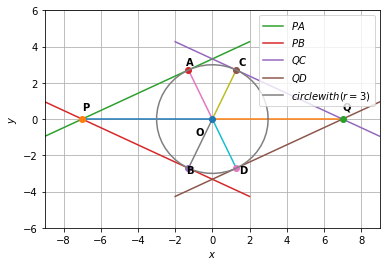
\includegraphics[width=\columnwidth]{FIGURE3.png}
    \caption{Tangent lines to circle of radius 3 units.}
    \label{fig:Tangent lines to circle of radius 3 units.}
\end{figure}
\end{document}
